\documentclass[12pt,a4paper,german]{report}
\usepackage{geometry}
\geometry{a4paper, top=25mm, left=25mm, right=25mm, bottom=30mm, headsep=10mm, footskip=12mm}
\usepackage[utf8]{inputenc}
\usepackage{titlesec}
\usepackage{blindtext}
\usepackage{hyperref}
\usepackage{babel}
\usepackage{titlepic}
\usepackage{graphicx}
\usepackage{algorithm}
\usepackage{amsmath}
\usepackage{mathptmx}
\usepackage[onehalfspacing]{setspace}
\usepackage[noend]{algpseudocode}
\graphicspath{ {./images/} }

\titleformat{\chapter}{\normalfont\huge\bfseries}{\thechapter.}{20pt}{\huge\bfseries}

%%%%%%%%%%%%%%%%%%%%%%%%%%%%%%%%%%%%%%%%%%%%%%%%%%%%%%%%%%%%%%%%%%%%%%%%%%%%%%%%

\begin{document}

\begin{titlepage}
  \centering
  
\includegraphics[width=0.05\textwidth]{ktzh}\par
  {\scshape\LARGE Berufsmaturitätsschule Zürich \par}
  \vspace{0.25cm}
  {\scshape\Large Berufsmaturitätsarbeit \par}
  {\scshape Technik,  Architektur,  Life  Sciences \par}
  \vspace{0.50cm}
  {\huge\bfseries Pathfinding-Algorithmen: Einführung und Vergleich mittels einer Webapplikation \par}
  \vspace{0.5cm}
  Oberthema: \textsc{Mobilität} \\
  \vspace{0.5cm}
  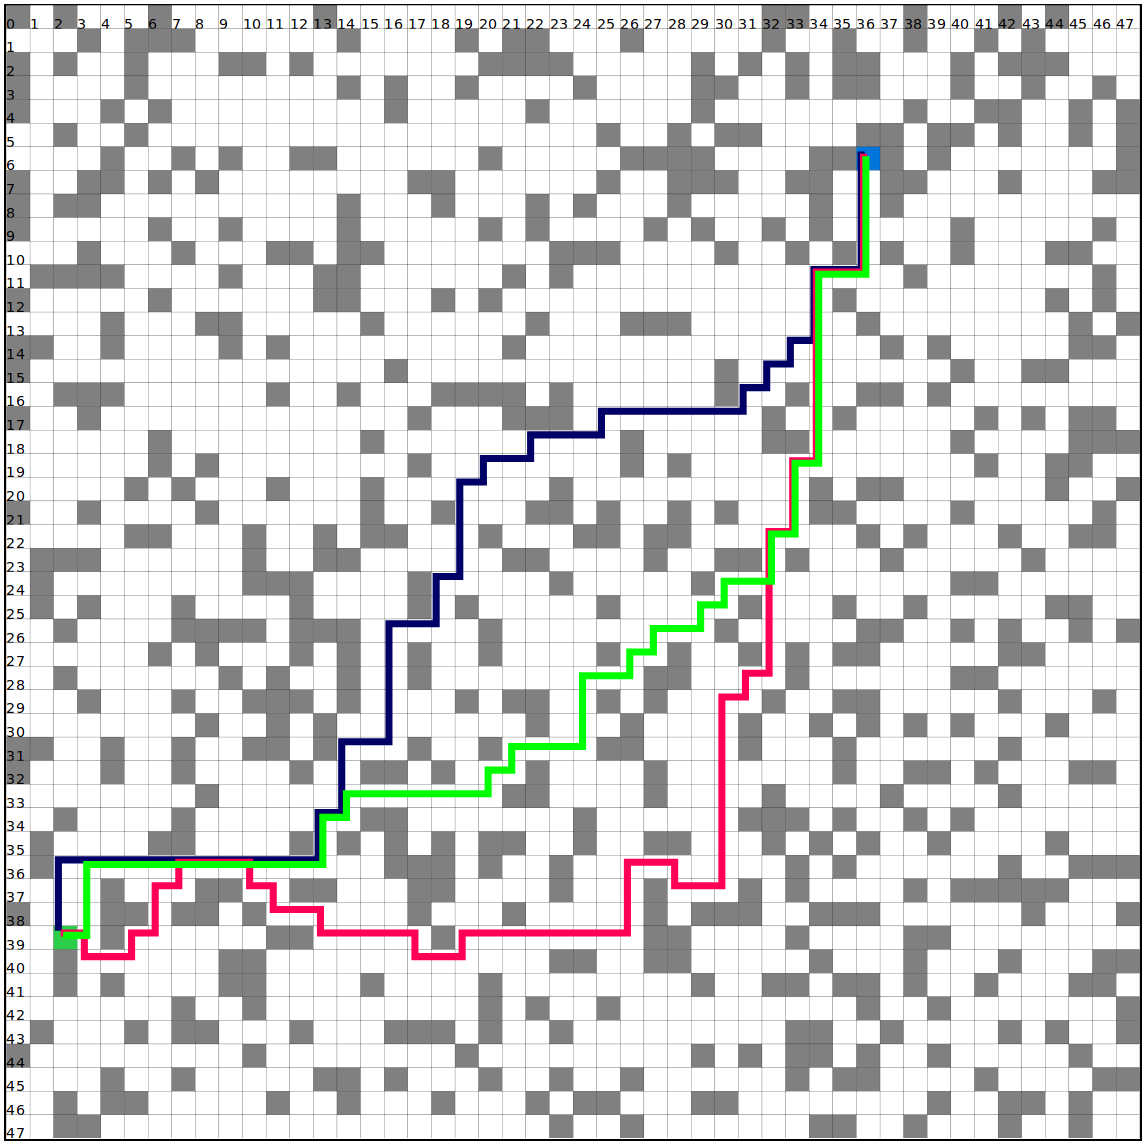
\includegraphics[width=0.65\textwidth]{cover2}\par
  \vspace{0.5cm}
  \begin{tabular}[t]{c@{\extracolsep{4em}}c} 
  \large\textsc{Adrian Stoop} & \large\textsc{Severin Fürbringer} \\ 
  adrian-stoop@gmx.ch & severin@fsfe.org\\
  EVT18a & EVT18a
  \end{tabular}
  \vfill
  \vspace{0.25cm}
  \large\textsc{Dr. Jürg Pöttinger}\\
  \normalsize{Begleitperson}
  \vspace{0.25cm}
  \vfill
  {1. Februar, 2019 \par}
\end{titlepage}


\renewcommand{\abstractname}{Abstract}
\begin{abstract}
Pathfinding-Algorithmen sind Programmabläufe, welche in der Wirtschaft in vielen Anwendungen vorkommen, wie zum Beispiel in Video Spielen, Simulationen oder der Automobilindustrie. 
Im Rahmen dieser Berufsmaturitätsarbeit wird eine Webapplikation entwickelt, die den Benutzer in das Thema der Pathfinder-Algorithmen einführt und einen interaktiven Vergleich von drei ausgewählten Pathfindern ermöglicht und dazu Messungen mit drei Merkmalen macht. Im Rahmen der Arbeit wählen wir den A*, BestFirst, und BreadthFirstFinder.
Die Webapplikation generiert für den Vergleich ein Zufallslabyrinth, markiert Start- und Endpünkte und lässt mehrere Vergleiche in Serie geschaltet zu.
Mithilfe des Pathfinder-Vergleichers werden im Rahmen der Arbeit auch Statistiken erstellt und ausgewertet und im schriftlichen Teil die Funktionsweisen der Pathfinder erläutert.
\\
  Die Webapplikation ist unter \url{https://bma.fuerbringer.info} zugänglich. Der dazugehörige Quellcode ist frei unter \url{https://github.com/fuerbringer/bma} erhältlich.
\end{abstract}


\tableofcontents{}

% START THESIS CONTENT
%%%%%%%%%%%%%%%%%%%%%%%%%%%%%%%%%%%%%%%%%%%%%%%%%%%%%%%%%%%%%%%%%%%%%%%%%%%%%%%%

\chapter{Einleitung}

%%%%%%%%%%%%%%%%%%%%%%%%%%%%%%%%%%%%%%%%%%%%%%%%%%%%%%%%%%%%%%%%%%%%%%%%%%%%%%%%
\chapter{Realisierung}
\section{Konzept}
Die Konzipierung dieser Webapplikation verlangte einige technische und gestalterische Entscheidungen. 
Einerseits musste die Programmiersprache und Struktur der Applikation geplant werden und andererseits auch das eigentliche Aussehen der Benutzeroberfläche der Webapplikation. 
Auf diese zwei wesentlichen Aspekte wird in diesem Abschnitt eingegangen.
\subsection{Pathfinding.js}
Eine korrekte Implementation der ausgewählten Pathfinder sind Voraussetzung für das Projekt. 
Daher wurde, um diese Voraussetzung zu erfüllen, eine frei verfügbare Implementation PathFinding.js \cite{pfjs} verschiedener Pathfinder ausgewählt.
\subsection{Programmierung}
Die vorhandenen Fachkenntnisse und Erfahrungen schlugen für die Implementierung entweder PHP oder JavaScript als mögliche Programmiersprachen vor. 
Zum Entscheid massgebend war, dass die Programmbibliothek PathFinding.js \cite{pfjs}, welche in unserer Arbeit eine wichtige Rolle spielt, in JavaScript implementiert wurde. 
Durch den Einsatz von JavaScript im Front-End und im Back-End, wäre es möglich die Pathfinder Berechnungen beliebig auf dem Rechner des Nutzers und auch auf dem Rechner des Servers auszuführen. 
Folgend werden die wichtigsten Technologien unserer Webapplikation aufgelistet\footnote{Eine komplette Auflistung inklusive der abhängenden Programmbibliotheken macht wenig Sinn, vor allem da unser Quellcode frei ersichtlich ist.}.

\begin{description}
  \item [Programmiersprache] JavaScript mit Einbindung von PathFinding.js \cite{pfjs}
  \item [Webserver-Software] Express\footnote{Express Webserver für Node Webapplikationen, \url{https://expressjs.com/}, Stand: \today}
  \item [Webhosting] Vultr\footnote{Vultr - The Infrastructure Cloud™, \url{https://vultr.com/}, Stand: \today}
  \item [Quellcode-Hosting] GitHub\footnote{GitHub, \url{https://github.com/}, Stand: \today}. Der Quellcode unser Webapplikation ist frei unter \url{https://github.com/fuerbringer/bma} zugänglich.
\end{description}

\subsection{Konzipierung der Benutzeroberfläche}
\begin{figure}
  \centering
  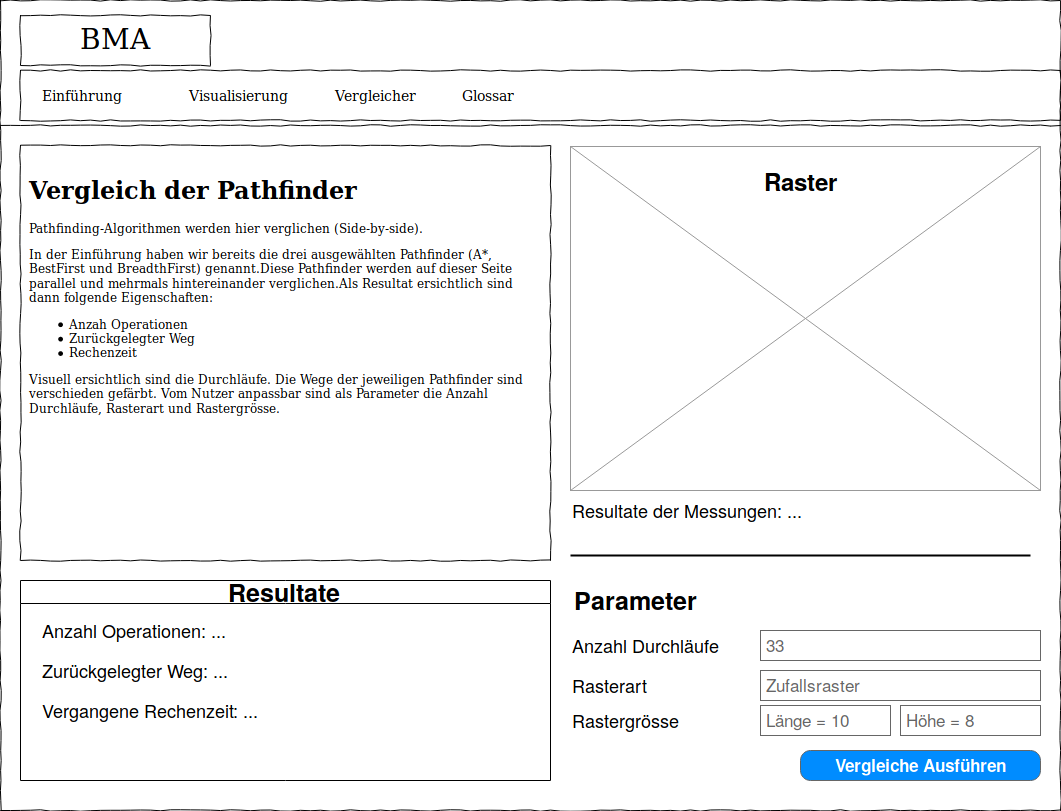
\includegraphics[width=16cm]{konzept1}
  \caption[Benutzeroberflächenkonzept des Pathfinder-Vergleichers.]{Benutzeroberflächenkonzept. Quelle: Eigenleistung}
  \label{fig:gui_konzept}
\end{figure}

%%%%%%%%%%%%%%%%%%%%%%%%%%%%%%%%%%%%%%%%%%%%%%%%%%%%%%%%%%%%%%%%%%%%%%%%%%%%%%%%
\chapter{Schluss}
\blindtext

% END THESIS CONTENT
%%%%%%%%%%%%%%%%%%%%%%%%%%%%%%%%%%%%%%%%%%%%%%%%%%%%%%%%%%%%%%%%%%%%%%%%%%%%%%%%

\clearpage

\begin{thebibliography}{9}
\bibitem{pfjs}
  Xueqiao Xu et al.,
  \textit{PathFinding.js},
  \url{https://github.com/qiao/PathFinding.js},
  Quellcode auf GitHub,
  Letzter Aufruf: \today
\bibitem{cuishi2011}
  Xiao, Cui; Hao Shi,
  \textit{A*-based Pathfinding in Modern Computer Games},
  IJCSNS International Journal of Computer Science and Network Security, VOL.11 No.1,
  Januar 2011.
\bibitem{bma}
  Fürbringer, Severin; Stoop, Adrian,
  \textit{BMA Quellcode},
  \url{https://github.com/fuerbringer/bma},
  \today
\bibitem{bmaonline}
  Fürbringer, Severin; Stoop, Adrian,
  \textit{BMA-Webapplikation},
  \url{https://bma.fuerbringer.info},
  \today
\end{thebibliography}


\listoffigures

\end{document}
